\tikzset{every picture/.style={line width=0.75pt}} %set default line width to 0.75pt        

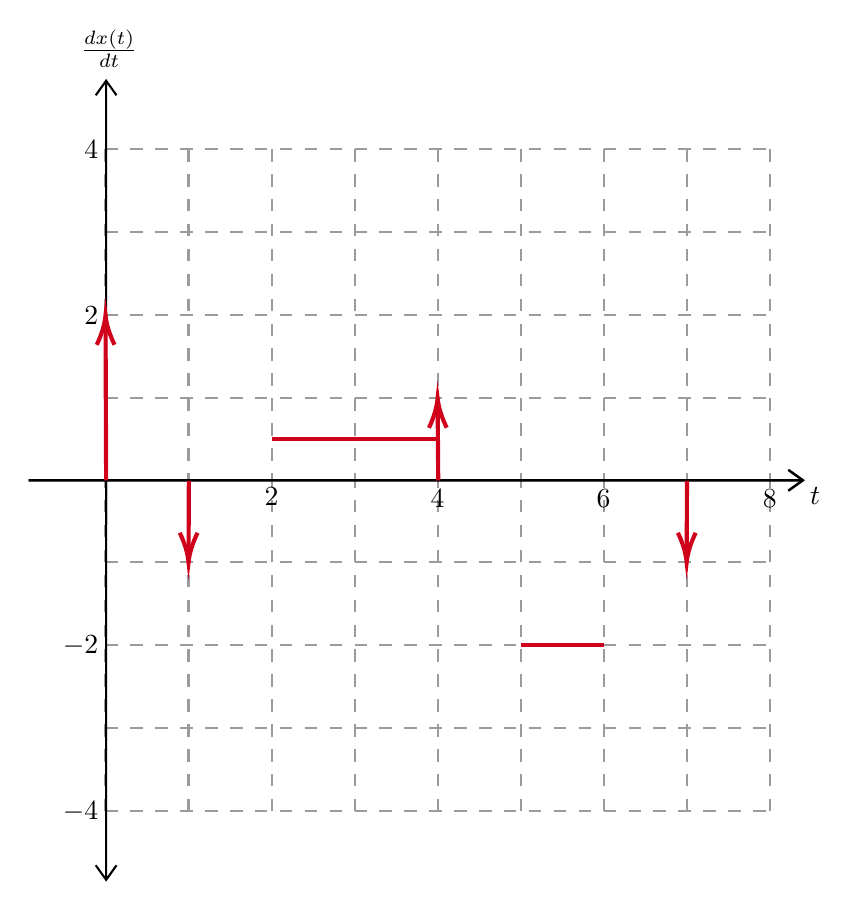
\begin{tikzpicture}[x=0.75pt,y=0.75pt,yscale=-1,xscale=1]
%uncomment if require: \path (0,757); %set diagram left start at 0, and has height of 757

%Shape: Grid [id:dp309180394936597] 
\draw  [draw opacity=0][dash pattern={on 4.5pt off 4.5pt}] (181,451) -- (502,451) -- (502,291) -- (181,291) -- cycle ; \draw  [color={rgb, 255:red, 155; green, 155; blue, 155 }  ,draw opacity=1 ][dash pattern={on 4.5pt off 4.5pt}] (181,451) -- (181,291)(221,451) -- (221,291)(261,451) -- (261,291)(301,451) -- (301,291)(341,451) -- (341,291)(381,451) -- (381,291)(421,451) -- (421,291)(461,451) -- (461,291)(501,451) -- (501,291) ; \draw  [color={rgb, 255:red, 155; green, 155; blue, 155 }  ,draw opacity=1 ][dash pattern={on 4.5pt off 4.5pt}] (181,451) -- (502,451)(181,411) -- (502,411)(181,371) -- (502,371)(181,331) -- (502,331) ; \draw  [color={rgb, 255:red, 155; green, 155; blue, 155 }  ,draw opacity=1 ][dash pattern={on 4.5pt off 4.5pt}]  ;
%Shape: Grid [id:dp1199375004666744] 
\draw  [draw opacity=0][dash pattern={on 4.5pt off 4.5pt}] (181,132) -- (502,132) -- (502,292) -- (181,292) -- cycle ; \draw  [color={rgb, 255:red, 155; green, 155; blue, 155 }  ,draw opacity=1 ][dash pattern={on 4.5pt off 4.5pt}] (181,132) -- (181,292)(221,132) -- (221,292)(261,132) -- (261,292)(301,132) -- (301,292)(341,132) -- (341,292)(381,132) -- (381,292)(421,132) -- (421,292)(461,132) -- (461,292)(501,132) -- (501,292) ; \draw  [color={rgb, 255:red, 155; green, 155; blue, 155 }  ,draw opacity=1 ][dash pattern={on 4.5pt off 4.5pt}] (181,132) -- (502,132)(181,172) -- (502,172)(181,212) -- (502,212)(181,252) -- (502,252) ; \draw  [color={rgb, 255:red, 155; green, 155; blue, 155 }  ,draw opacity=1 ][dash pattern={on 4.5pt off 4.5pt}]  ;
%Shape: Axis 2D [id:dp9049348521282261] 
\draw  (144,291.6) -- (517,291.6)(181.3,99) -- (181.3,313) (510,286.6) -- (517,291.6) -- (510,296.6) (176.3,106) -- (181.3,99) -- (186.3,106)  ;
%Shape: Axis 2D [id:dp3810174740882728] 
\draw  (144,291.4) -- (517,291.4)(181.3,484) -- (181.3,270) (510,296.4) -- (517,291.4) -- (510,286.4) (176.3,477) -- (181.3,484) -- (186.3,477)  ;
%Straight Lines [id:da23465514220892947] 
\draw [color={rgb, 255:red, 208; green, 2; blue, 27 }  ,draw opacity=1 ][line width=1.5]    (181.3,291.6) -- (181.01,215) ;
\draw [shift={(181,212)}, rotate = 89.78] [color={rgb, 255:red, 208; green, 2; blue, 27 }  ,draw opacity=1 ][line width=1.5]    (14.21,-4.28) .. controls (9.04,-1.82) and (4.3,-0.39) .. (0,0) .. controls (4.3,0.39) and (9.04,1.82) .. (14.21,4.28)   ;
%Straight Lines [id:da9635494729893386] 
\draw [color={rgb, 255:red, 208; green, 2; blue, 27 }  ,draw opacity=1 ][line width=1.5]    (221.15,291.8) -- (221.01,328) ;
\draw [shift={(221,331)}, rotate = 270.22] [color={rgb, 255:red, 208; green, 2; blue, 27 }  ,draw opacity=1 ][line width=1.5]    (14.21,-4.28) .. controls (9.04,-1.82) and (4.3,-0.39) .. (0,0) .. controls (4.3,0.39) and (9.04,1.82) .. (14.21,4.28)   ;
%Straight Lines [id:da8624510645837334] 
\draw [color={rgb, 255:red, 208; green, 2; blue, 27 }  ,draw opacity=1 ][line width=1.5]    (341.15,271.8) -- (261.15,271.8) ;
%Straight Lines [id:da08847746311409221] 
\draw [color={rgb, 255:red, 208; green, 2; blue, 27 }  ,draw opacity=1 ][line width=1.5]    (341.3,291.6) -- (341.02,255) ;
\draw [shift={(341,252)}, rotate = 89.57] [color={rgb, 255:red, 208; green, 2; blue, 27 }  ,draw opacity=1 ][line width=1.5]    (14.21,-4.28) .. controls (9.04,-1.82) and (4.3,-0.39) .. (0,0) .. controls (4.3,0.39) and (9.04,1.82) .. (14.21,4.28)   ;
%Straight Lines [id:da17568992650795978] 
\draw [color={rgb, 255:red, 208; green, 2; blue, 27 }  ,draw opacity=1 ][line width=1.5]    (421,371) -- (381,371) ;
%Straight Lines [id:da7395813657008669] 
\draw [color={rgb, 255:red, 208; green, 2; blue, 27 }  ,draw opacity=1 ][line width=1.5]    (461.15,291.8) -- (461.01,328) ;
\draw [shift={(461,331)}, rotate = 270.22] [color={rgb, 255:red, 208; green, 2; blue, 27 }  ,draw opacity=1 ][line width=1.5]    (14.21,-4.28) .. controls (9.04,-1.82) and (4.3,-0.39) .. (0,0) .. controls (4.3,0.39) and (9.04,1.82) .. (14.21,4.28)   ;

% Text Node
\draw (182.72,94) node [anchor=south] [inner sep=0.75pt]    {$\frac{dx( t)}{dt}$};
% Text Node
\draw (519,293.4) node [anchor=north west][inner sep=0.75pt]    {$t$};
% Text Node
\draw (341,294.4) node [anchor=north] [inner sep=0.75pt]    {$4$};
% Text Node
\draw (421,294.4) node [anchor=north] [inner sep=0.75pt]    {$6$};
% Text Node
\draw (261,293.4) node [anchor=north] [inner sep=0.75pt]    {$2$};
% Text Node
\draw (501,294.4) node [anchor=north] [inner sep=0.75pt]    {$8$};
% Text Node
\draw (179,212) node [anchor=east] [inner sep=0.75pt]    {$2$};
% Text Node
\draw (179,132) node [anchor=east] [inner sep=0.75pt]    {$4$};
% Text Node
\draw (179,371) node [anchor=east] [inner sep=0.75pt]    {$-2$};
% Text Node
\draw (179,451) node [anchor=east] [inner sep=0.75pt]    {$-4$};


\end{tikzpicture}
